\documentclass[]{beamer}
\usepackage{beamerthemesplit}
\usepackage{graphics}
\usepackage{pstricks}
\usepackage{graphicx}
\usepackage{hyperref}
\usepackage{subfigure}
\usepackage{multirow}
\usepackage{listings}
\usepackage{courier}
\usepackage{xspace}
\usepackage{tikz}

%\lstset{escapechar=@,style=customc}


\mode<presentation>
{ \usetheme{Boadilla}
  \setbeamercovered{transparent}
  \setbeamertemplate{items}[circle]
  \setbeamertemplate{theorems}[numbered]
  \setbeamertemplate{footline}[frame number]
}
 
%\useinnertheme[shadow=true]{rounded}
\useoutertheme{shadow}
\usecolortheme{whale}

\newcommand\blfootnote[1]{
  \begingroup
  \renewcommand\thefootnote{}\footnote{#1}
  \addtocounter{footnote}{-1}
  \endgroup
}

\mode
<all>

\title{C Programming}
\author{Wan-Lei Zhao}

\makeatletter
\DeclareRobustCommand\onedot{\futurelet\@let@token\@onedot}
\def\@onedot{\ifx\@let@token.\else.\null\fi\xspace}
\DeclareMathOperator*{\argmax}{argmax}
\makeatother

\begin{document}


\begin{frame}
   \begin{center}
    \vspace{24pt}
    \Huge\textbf{C Programming}\blfootnote{Email: wlzhao@xmu.edu.cn, copyrights are fully reserved by the author.}\\
     \Huge{Lecture 1: An Introduction and Overview on C}
      \begin{figure}
     	\begin{center}
     		
\includegraphics[width=0.3\linewidth]{figs/turingma.pdf}
     	\end{center}
     \end{figure}
    \vspace{36pt}
  \end{center}
  \begin{align*}
   \vspace{18pt}
      \large{\mbox{Lecturer:}~Dr.~\mbox{Wan-Lei~~Zhao}} \\
      \large{Spring~~Semester~~2022} \\
   \vspace{30pt}
  \end{align*}
\end{frame}

\definecolor{cornblue}{HTML}{6495ED}
\definecolor{navyblue}{HTML}{000080}
\definecolor{midnblue}{HTML}{191970}
\definecolor{lghtblue}{HTML}{B0C4DE}
\setbeamercolor{background}{fg=black, bg=lghtblue}
\setbeamercolor{palette primary}{fg=white, bg=lghtblue}
\setbeamercolor{palette secondary}{fg=black, bg=cornblue}
\setbeamercolor{palette tertiary}{fg=black, bg=lghtblue}
\setbeamercolor{palette quaternary}{fg=black, bg=lghtblue}
\setbeamercolor{frametitle}{fg=black, bg=white}
\definecolor{ballblue}{rgb}{0.13, 0.67, 0.8}
\definecolor{cornflowerblue}{rgb}{0.39,0.58,0.93}
\definecolor{babyblueeyes}{rgb}{0.63, 0.79, 0.95}

\setbeamertemplate{footline}
{
  \leavevmode%
  \hbox{%
  \begin{beamercolorbox}[wd=.275\paperwidth,ht=2.25ex,dp=1ex,center]{author in head/foot}%
    \usebeamerfont{author in head/foot}\insertshortauthor
  \end{beamercolorbox}%
  \begin{beamercolorbox}[wd=.44\paperwidth,ht=2.25ex,dp=1ex,center]{title in head/foot}%
    \usebeamerfont{title in head/foot}\insertshorttitle\hspace*{3em}
    \hspace*{1ex}
  \end{beamercolorbox}%
  \begin{beamercolorbox}[wd=.285\paperwidth,ht=2.25ex,dp=1ex,center]{date/foot}%
    \usebeamerfont{title in head/foot}\hspace*{2em}
    \insertframenumber{} / \inserttotalframenumber\hspace*{1ex}
  \end{beamercolorbox}}%
  \vskip0pt
}



% preset-listing options
\lstset{
  backgroundcolor=\color{white},   
  basicstyle=\footnotesize,    
  language=c,
  breakatwhitespace=false,         
  breaklines=true,                 % sets automatic line breaking
  captionpos=b,                    % sets the caption-position to bottom
  commentstyle=\color{ballblue},    % comment style
  extendedchars=true,              
  frame=single,                    % adds a frame around the code     
  keywordstyle=\color{blue},       % keyword style
  numbers=left,                    
  numbersep=5pt,                   
  numberstyle=\tiny\color{blue}, 
  rulecolor=\color{babyblueeyes},
  stepnumber=1,              
  stringstyle=\color{black},     % string literal style
  tabsize=4,                       % sets default tabsize to 4 spaces
  title=\lstname                   
}


\section{Syllabus}
\label{sec:sylla}
\begin{frame}<beamer>
    \frametitle{Outline}
    \tableofcontents[currentsection]
\end{frame}

\begin{frame}
	\frametitle{Syllabus}
	\begin{enumerate}
		\item {Primitive Data Types and Operations}
		\item {Sequential Control}
		\item {Selection Control clause: \textcolor{blue}{if-else} and \textcolor{blue}{switch}}
		\item {Loops Control clause: \textcolor{blue}{while}, \textcolor{blue}{do-while} and \textcolor{blue}{for}}
		\item {Functions: declaration, definition and calling}
		\item {Pre-compilation Command/Macros: \textcolor{blue}{\#ifdef}}
		\item {Array: declaration, definition and calling}
		\item {Structures: \textcolor{blue}{struct} and \textcolor{blue}{union}}
		\item {Pointers}
		\item {File Operations: read and write}
	\end{enumerate}
	\begin{itemize}
		\item {Performance Evaluation}
		\begin{itemize}
			\item {Final score=10\%{$\times$}Exerc.+30\%{$\times$}Quiz.+10\%{$\times$}Att.+50\%{$\times$}Exam}
		\end{itemize}
	\end{itemize}
\end{frame}


\begin{frame}
	\frametitle{Arrangement of this course}
\begin{itemize}
	\item {16 weeks${\times}$2 hours classes}
	\item {8 weeks${\times}$2 hours labs}
	\begin{itemize}
			\item {TA and I will be in the lab}
	\end{itemize}
	\item {Middle-term exam}
	\item {Doing final exam, both are held in the lab}
	\begin{itemize}
		\item {Multiple choices}	
		\item {Correct codes}
		\item {3-4 coding problems}
	\end{itemize}
	\item {\textcolor{red}{No cheating and no bargaining!}}
	\item {If you attend all my classes}
	\item {I ensure that you can learn a lot:)}
\end{itemize}
\end{frame}


\begin{frame}{Exercise Website}
\begin{itemize}
	\item{PTA: \url{https://pintia.cn/}}
\end{itemize}

%\begin{figure}
%\begin{center}
%	\includegraphics[width=0.5\linewidth]{figs/ta/pta.pdf}
%\end{center}	
%\end{figure}

\begin{enumerate}
	\item {Register with your email account}
	\item {You can type your codes, submit and compile}
	\item {You should print out the exact answer}
\end{enumerate}

\end{frame}
\section{All about Computer}
\label{sec:computer}
\begin{frame}<beamer>
    \frametitle{Outline}
    \tableofcontents[currentsection]
\end{frame}

\begin{frame}
\frametitle{About Computer (1)}
\begin{itemize}
	\item {What is computer?}
	\begin{itemize}
		\item {Machine for computation}
		\item {Essentially, no big difference from abacus}
		\item {In our history, we have several kinds of machines used for computing}
		\begin{itemize}
			\item {Abacus}
			\item {Difference engine}
			\item {Tide-predicting machine}
		\end{itemize}
	\end{itemize}
\end{itemize}
\begin{figure}
	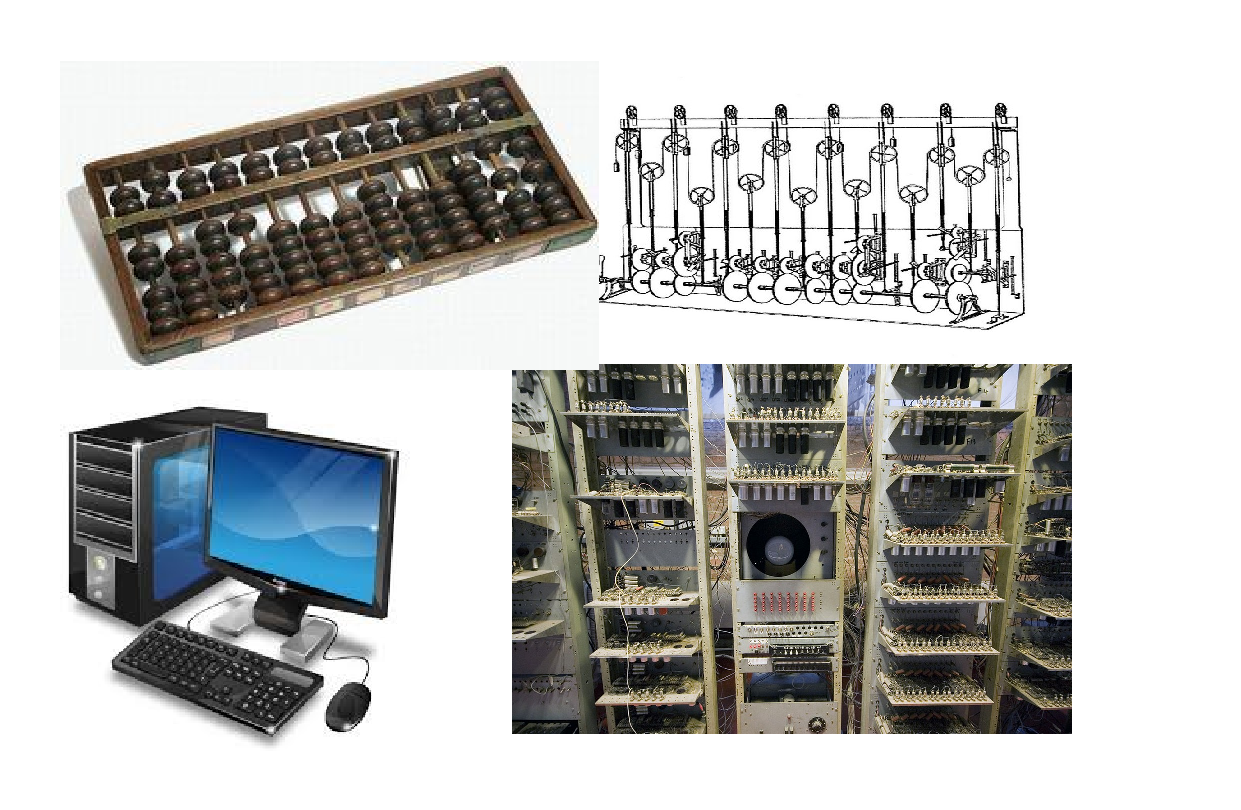
\includegraphics[width=0.5\linewidth]{figs/history_pcs.pdf}
\end{figure}
\end{frame}

\begin{frame}
\frametitle{About Computer (2): the model}
\begin{itemize}
	\item {What is computing}
	\begin{itemize}
		\item {Input data and needed operations}
		\item {Output the answer}
	\end{itemize}
	\begin{itemize}
		\item {This is actually the model proposed by \textbf{Alan Turing}}
	\end{itemize}
\end{itemize}
\begin{figure}
	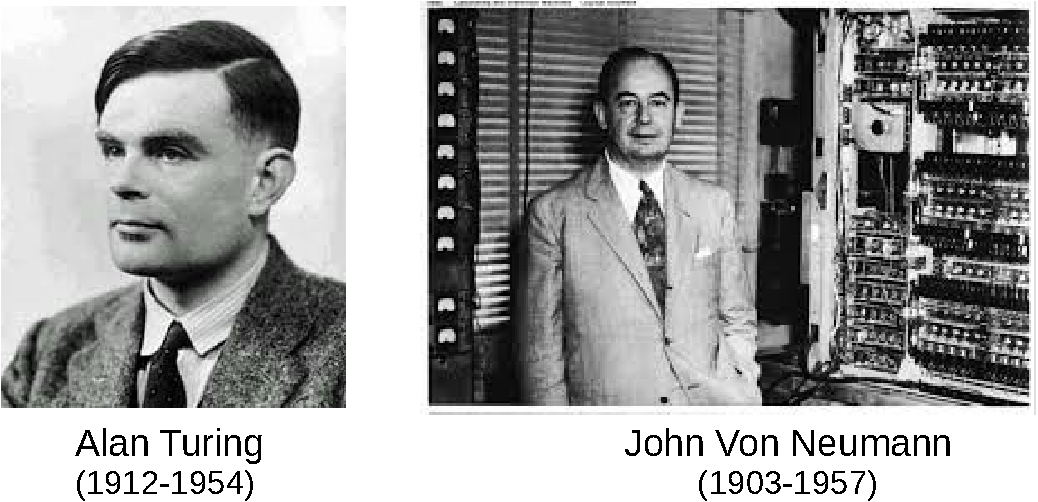
\includegraphics[width=0.8\linewidth]{figs/turing.pdf}
\end{figure}
\end{frame}

\begin{frame}
\frametitle{About Computer (3): the framework}
\begin{itemize}
	\item {Think aloud about the major components of a computer}
	\begin{itemize}
		\item {CPU: central processing unit}
		\item {Memory}
		\item {Hard disc}
		\item {Keyboard}
		\item {graphics card+Monitor/screen}
		\item {Music card+microphone+speaker}
		\item {Mouse}
	\end{itemize}
\end{itemize}
\begin{figure}
	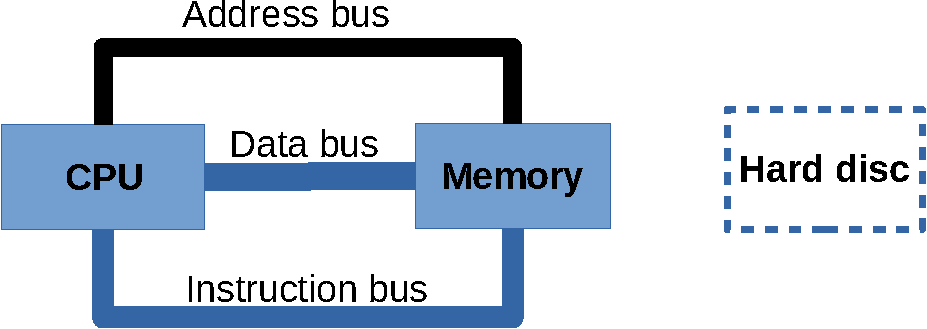
\includegraphics[width=0.7\linewidth]{figs/framework.pdf}
\end{figure}
\end{frame}

\begin{frame}
\frametitle{About Computer (4): the framework}
\begin{itemize}
	\item {Think aloud about the major components of a computer}
	\begin{itemize}
		\item {\textbf{CPU: central processing unit}}
		\item {\textbf{Memory}}
		\item {Hard disc}
		\item {Keyboard}
		\item {graphics card+Monitor/screen}
		\item {Music card+microphone+speaker}
		\item {Mouse}
	\end{itemize}
\end{itemize}
\begin{figure}
	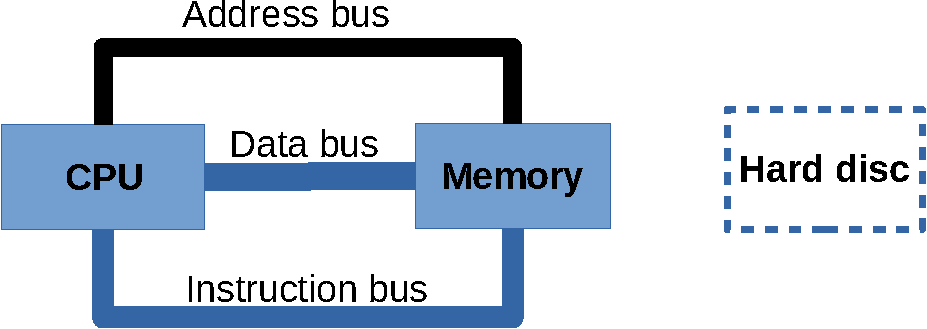
\includegraphics[width=0.7\linewidth]{figs/framework.pdf}
\end{figure}
\end{frame}

\begin{frame}
\frametitle{About Computer (5): who is who}
\begin{figure}
	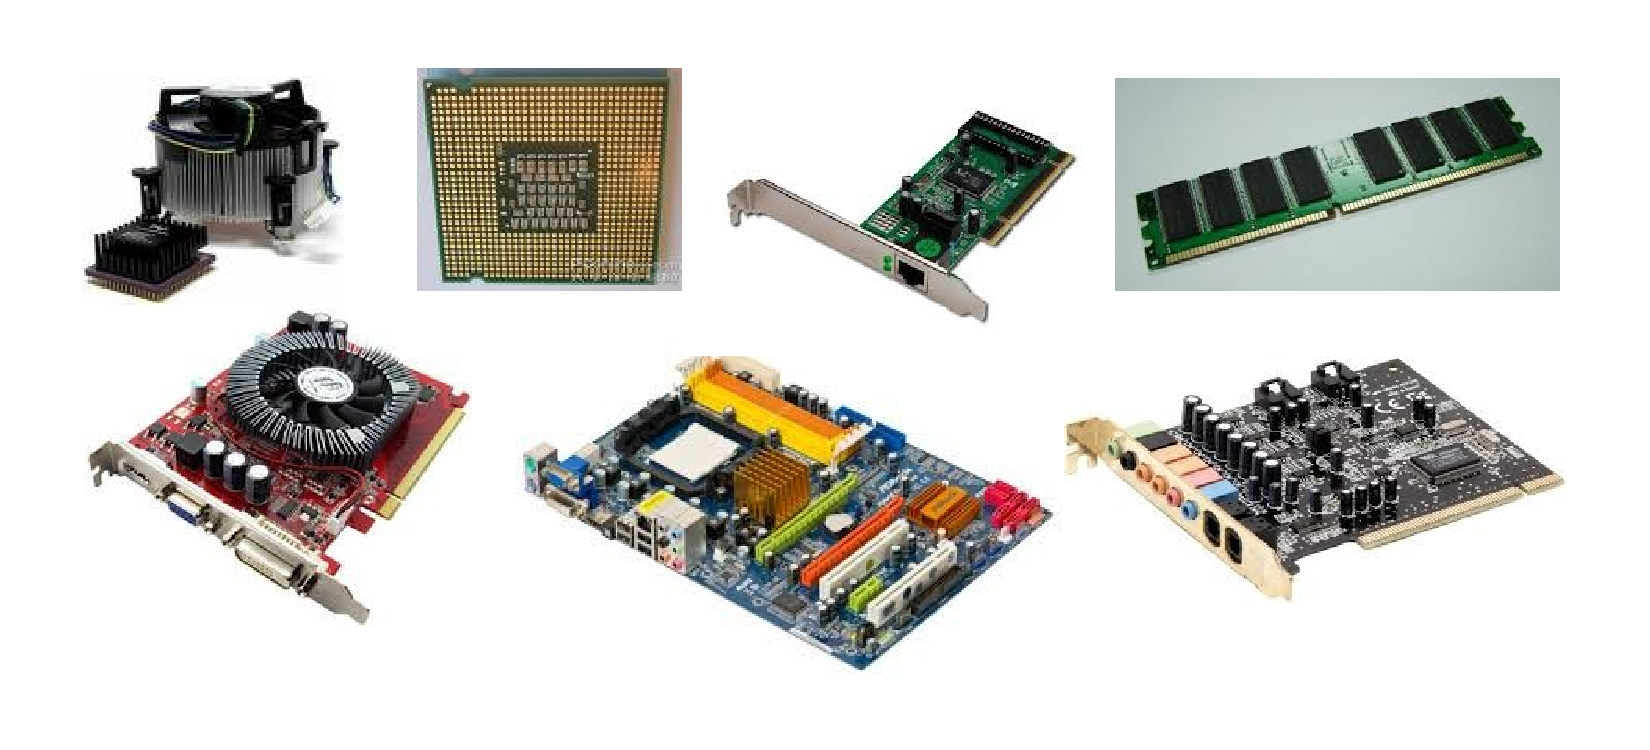
\includegraphics[width=0.85\linewidth]{figs/hardwares.pdf}
\end{figure}
\begin{itemize}
	\item {How many of them you can finger out?}
\end{itemize}
\end{frame}

\begin{frame}
\frametitle{About Computer (6): basic elements in Computer Chips}
\begin{figure}
	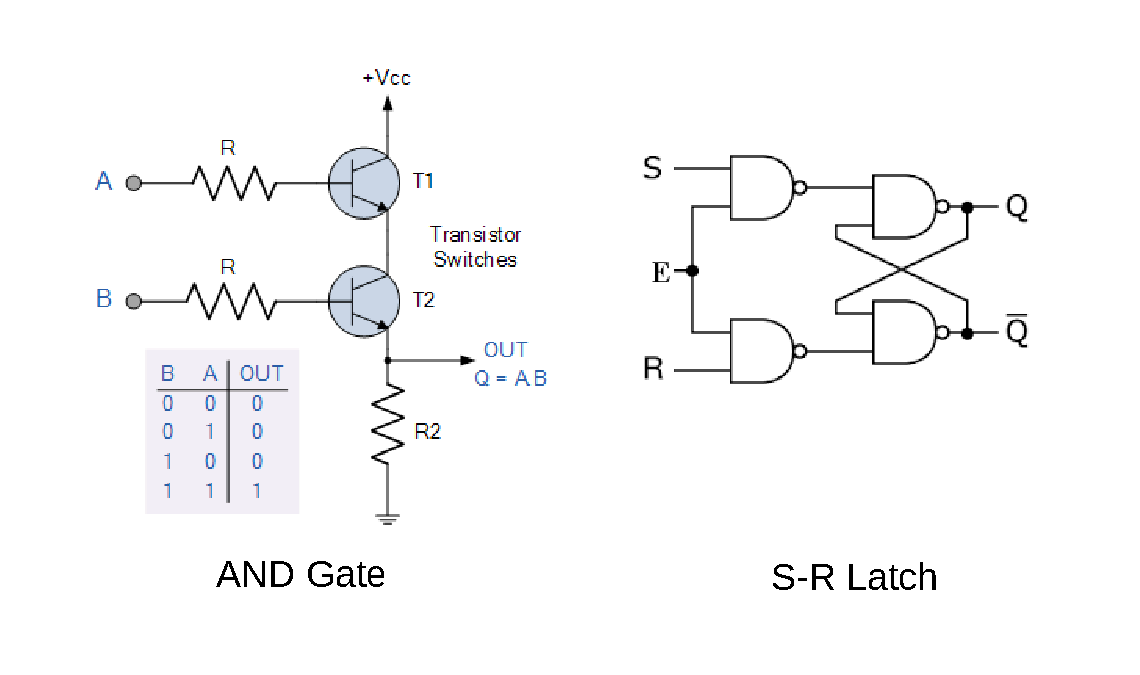
\includegraphics[width=0.6\linewidth]{figs/chips.pdf}
\end{figure}
\begin{itemize}
	\item {Despite the high complexity of VLSIC (very large scale integrated circuits)}
	\item {Only two basic elements are there}
	\item {One is gate, responsible for operations, main components for CPU}
	\item {Another is latch, in charge of memory, main components for memory}
\end{itemize}
\end{frame}
\section{Programming}
\label{sec:program}
\begin{frame}<beamer>
    \frametitle{Outline}
    \tableofcontents[currentsection]
\end{frame}

\begin{frame}
	\frametitle{Why programming? (1)}
	\begin{figure}
	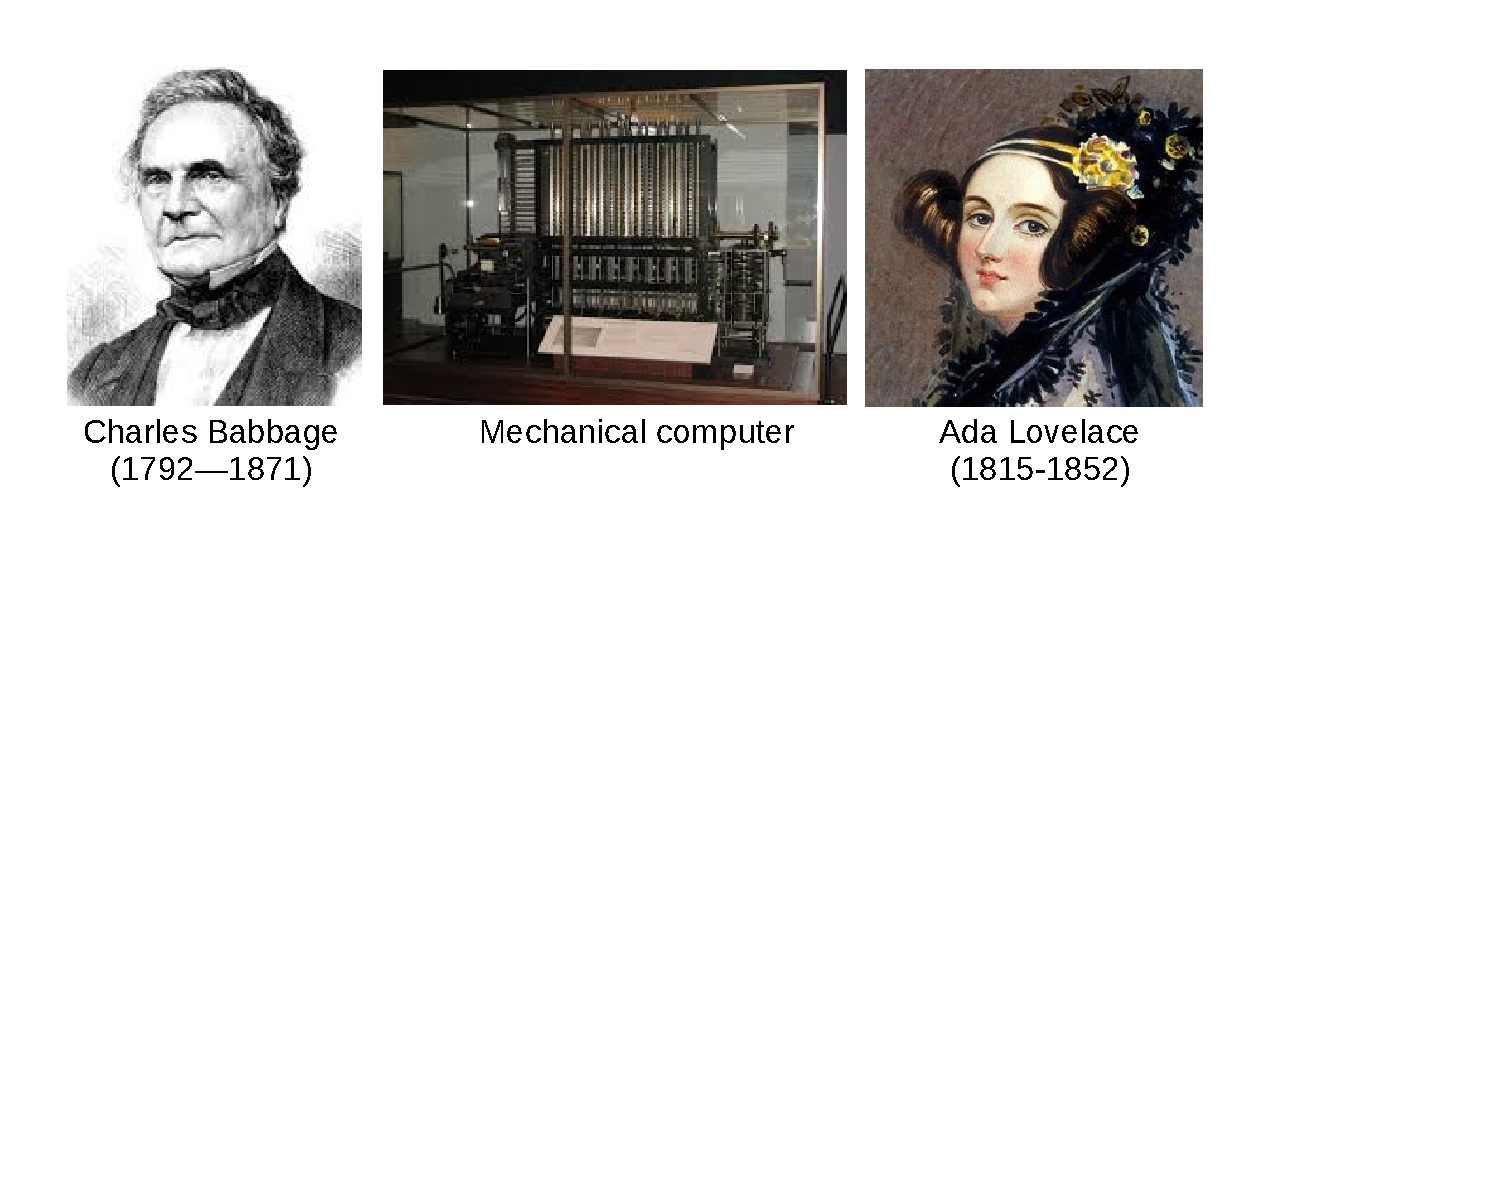
\includegraphics[width=0.85\linewidth]{figs/ada.pdf}
\end{figure}
\begin{itemize}
	\item {Ada is the first programmer}
	\item {A language is named after her to memorize her contribution}
\end{itemize}
\end{frame}

\begin{frame}
	\frametitle{Why programming? (2)}
	\begin{figure}
	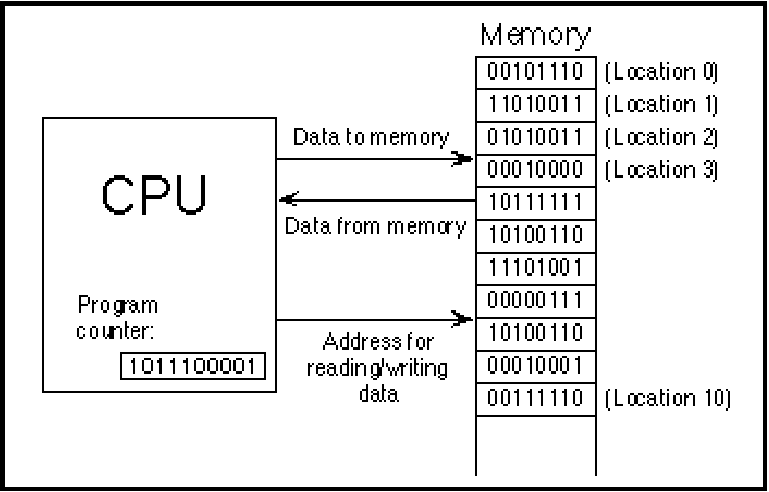
\includegraphics[width=0.65\linewidth]{figs/workflow.pdf}
\end{figure}
\begin{itemize}
	\item {Instructions and data fetch from memory to CPU for processing}
	\item {The results are returned back to memory}
\end{itemize}
\end{frame}

\begin{frame}
	\frametitle{Why High Level Programming Language? (1)}
\begin{figure}
	
\includegraphics[width=0.75\linewidth]{figs/talk2pc.pdf}
\end{figure}
\begin{itemize}
	\item {Natural language is the media that we communicate with each other}
	\item {Computer language is the media that we communicate with computer}
	\item {We should use the language that computer could understand}
	\item {At least, we need an \textcolor{red}{interpreter/translator}}
\end{itemize}
\end{frame}

\begin{frame}
	\frametitle{Why High Level Programming Language? (2)}
	\begin{figure}
	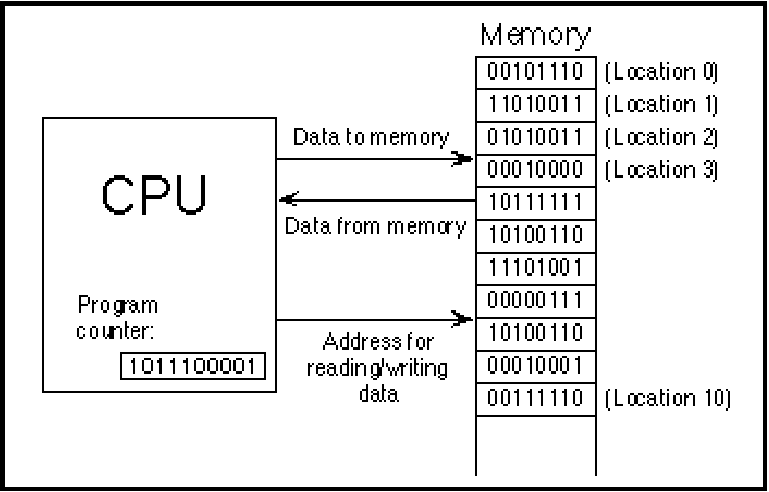
\includegraphics[width=0.65\linewidth]{figs/workflow.pdf}
\end{figure}
\begin{itemize}
	\item {Instructions are binary codes}
	\item {Machine only accepts/understands binary codes}
\end{itemize}
\end{frame}

\begin{frame}
	\frametitle{Why Programming Language? (3)}
\begin{columns}
\begin{column}{0.45\linewidth}
\begin{enumerate}
	\item {010101 0000 0011}
	\item {010101 0001 0101}
	\item {101010 0000 0001}
	\item {010101 0000 1011}
\end{enumerate}
\end{column}
\end{columns}
\end{frame}

\begin{frame}
	\frametitle{Why Programming Language? (4)}
\begin{columns}
\begin{column}{0.45\linewidth}
\begin{enumerate}
	\item {010101 0000 0011}
	\item {010101 0001 0101}
	\item {101010 0000 0001}
	\item {010101 0000 1011}
\end{enumerate}
\end{column}
\begin{column}{0.45\linewidth}
\vspace{-0.1in}
\begin{enumerate}
	\item {MOV D1 0011}
	\item {MOV D2 0101}
	\item {ADD D1 D2}
	\item {MOV D1 A1}
\end{enumerate}
\end{column}
\end{columns}
\vspace{0.2in}
\begin{itemize}
	\item {For the convenience of operation, binary instructions are denoted with readable symbols}
\end{itemize}

\end{frame}

\begin{frame}
	\frametitle{Why Programming Language? (5)}
\begin{columns}
\begin{column}{0.4\linewidth}
\begin{itemize}
	\item {Machine code}
\end{itemize}
\begin{enumerate}
	\item {010101 0000 0011}
	\item {010101 0001 0101}
	\item {101010 0000 0001}
	\item {010101 0000 1011}
\end{enumerate}
\end{column}
\begin{column}{0.3\linewidth}
\vspace{-0.1in}
\begin{itemize}
	\item {Assembly}
\end{itemize}
\begin{enumerate}
	\item {MOV D1 0011}
	\item {MOV D2 0101}
	\item {ADD D1 D2}
	\item {MOV D1 A1}
\end{enumerate}
\end{column}
\begin{column}{0.25\linewidth}
\vspace{-0.1in}
\begin{itemize}
	\item {High level language}
\end{itemize}
\begin{enumerate}
	\item {a=3+5;}
\end{enumerate}
\end{column}
\end{columns}
\end{frame}

\begin{frame}
	\frametitle{Why Programming Language? (6)}
\begin{figure}
	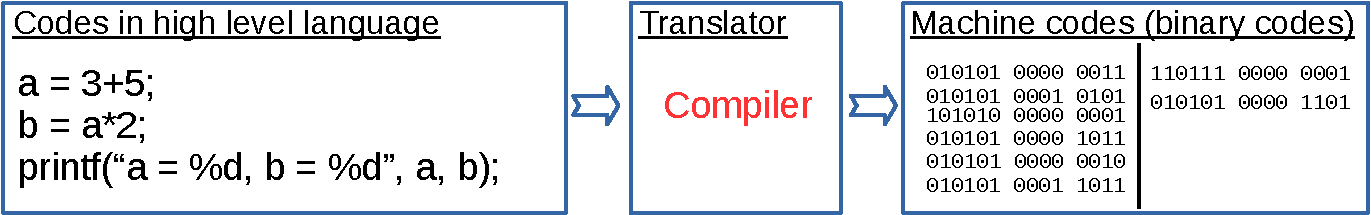
\includegraphics[width=0.95\linewidth]{figs/compil.pdf}
\end{figure}
\begin{itemize}
	\item {We write a \textcolor{red}{text} file in specified format (grammar)}
	\item {These are instructions that we basically understand}
	\item {The \textcolor{red}{translator} converts the text instructions into machine codes}
	\item {Machine then runs these binary codes one by one}
	\item {Different \textcolor{red}{translator}s lead to different programming languages}
	\item {Which also regulate different grammars}
	\item {C is such kind of high level language}
\end{itemize}
\end{frame}

\begin{frame}
	\frametitle{The life-time of a computer program}
\begin{figure}
	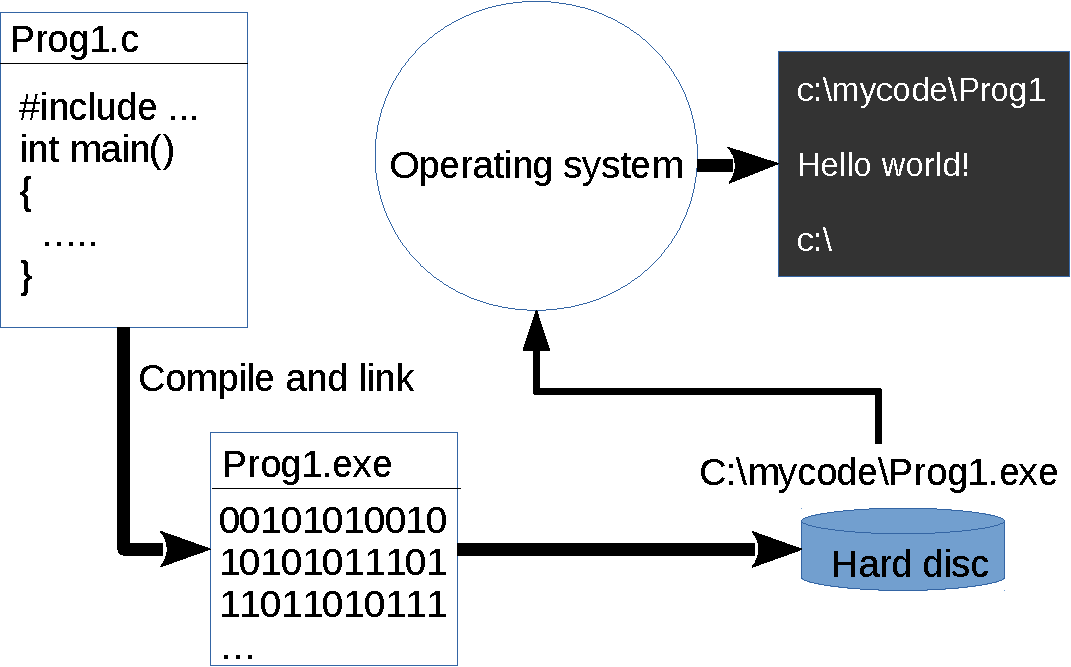
\includegraphics[width=0.95\linewidth]{figs/life-tm.pdf}
\end{figure}
\end{frame}
\section{Basics about C Programming}
\label{sec:basics}
\begin{frame}<beamer>
    \frametitle{Outline}
    \tableofcontents[currentsection]
\end{frame}

\begin{frame}
	\frametitle{Brief History about C}
	\vspace{-0.1in}
\begin{figure}
	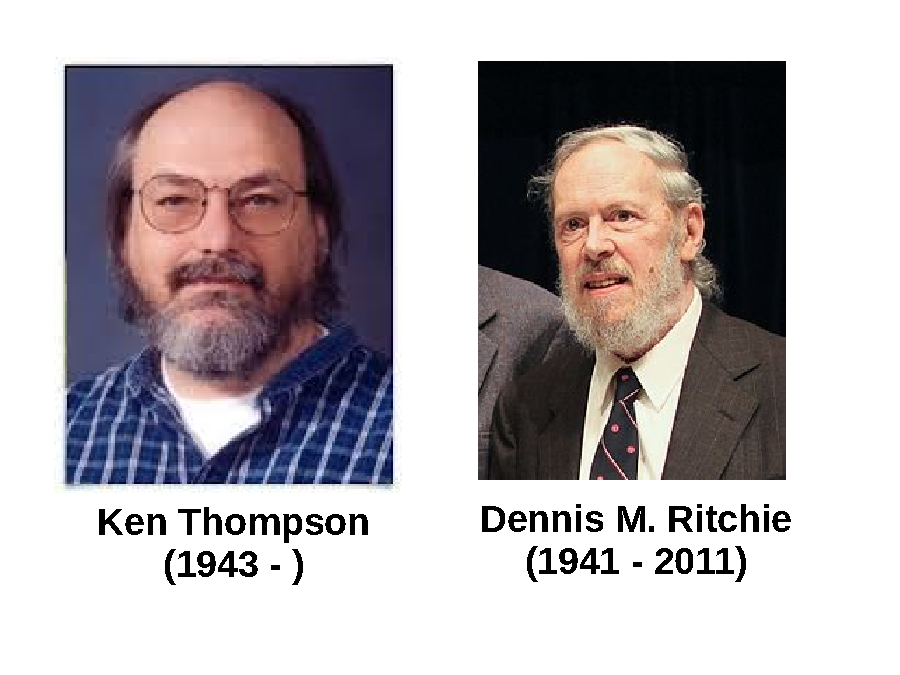
\includegraphics[width=0.5\linewidth]{figs/cuunix.pdf}
\end{figure}
\begin{itemize}
	\item {C is born in AT\&T Bell Labs along with UNIX}
	\item {The developer Dennis Ritchie and Ken Thompson were awarded with Turing Award}
	\item {C is simple:), versatile and highly efficient (70\% of assembly language efficiency)}
	\item {UNIX is one of the most stable operating systems so far developed}
\end{itemize}
\end{frame}

\begin{frame}[fragile]
	\frametitle{Your first program in C (1)}
\begin{lstlisting}[language=c]
#include <stdio.h>
int main()
{  /*start of a block*/
    printf("Hello world!\n"); /*call function 'printf'*/
    return 0;                 /*return '0' back*/
} /*end of a block*/
\end{lstlisting}
\vspace{-0.15in}
\begin{itemize}
		\item {``\#include $<$stdio.h$>$'' states that we want to use \textcolor{red}{function} defined in ``stdio.h'' }
		\item {Our code is encapsulated in a function called ``\textbf{main()}''}
		\item {In the main bordy of the function}
		\item {We output ``Hello world!'' to the screen}
		\item {``\textcolor{red}{printf()}'' is a function \textcolor{red}{defined} in ``stdio.h''}
		\item {\textcolor{blue}{include}, \textcolor{blue}{int} and \textcolor{blue}{return} are reserved keywords}
	\end{itemize}

\end{frame}


\begin{frame}[fragile]
	\frametitle{Your first program in C (2)}
\begin{lstlisting}[language=c]
#include <stdio.h>
int main()
{  
    printf("Hello world 1!\n"); 
    printf("Hello world 2!\n"); 
    printf("Hello world 3!\n"); 
    return 0;                 
} 
\end{lstlisting}
[Output]
\begin{lstlisting}[language=c]
   Hello world 1!
   Hello world 2!
   Hello world 3!           
\end{lstlisting}
\vspace{-0.15in}
\begin{itemize}
		\item {Codes are executed \textcolor{red}{from top to bottom}}
\end{itemize}

\end{frame}

\begin{frame}
	\frametitle{Popularity of C in recent decade}
	\vspace{-0.1in}
	\begin{figure}
		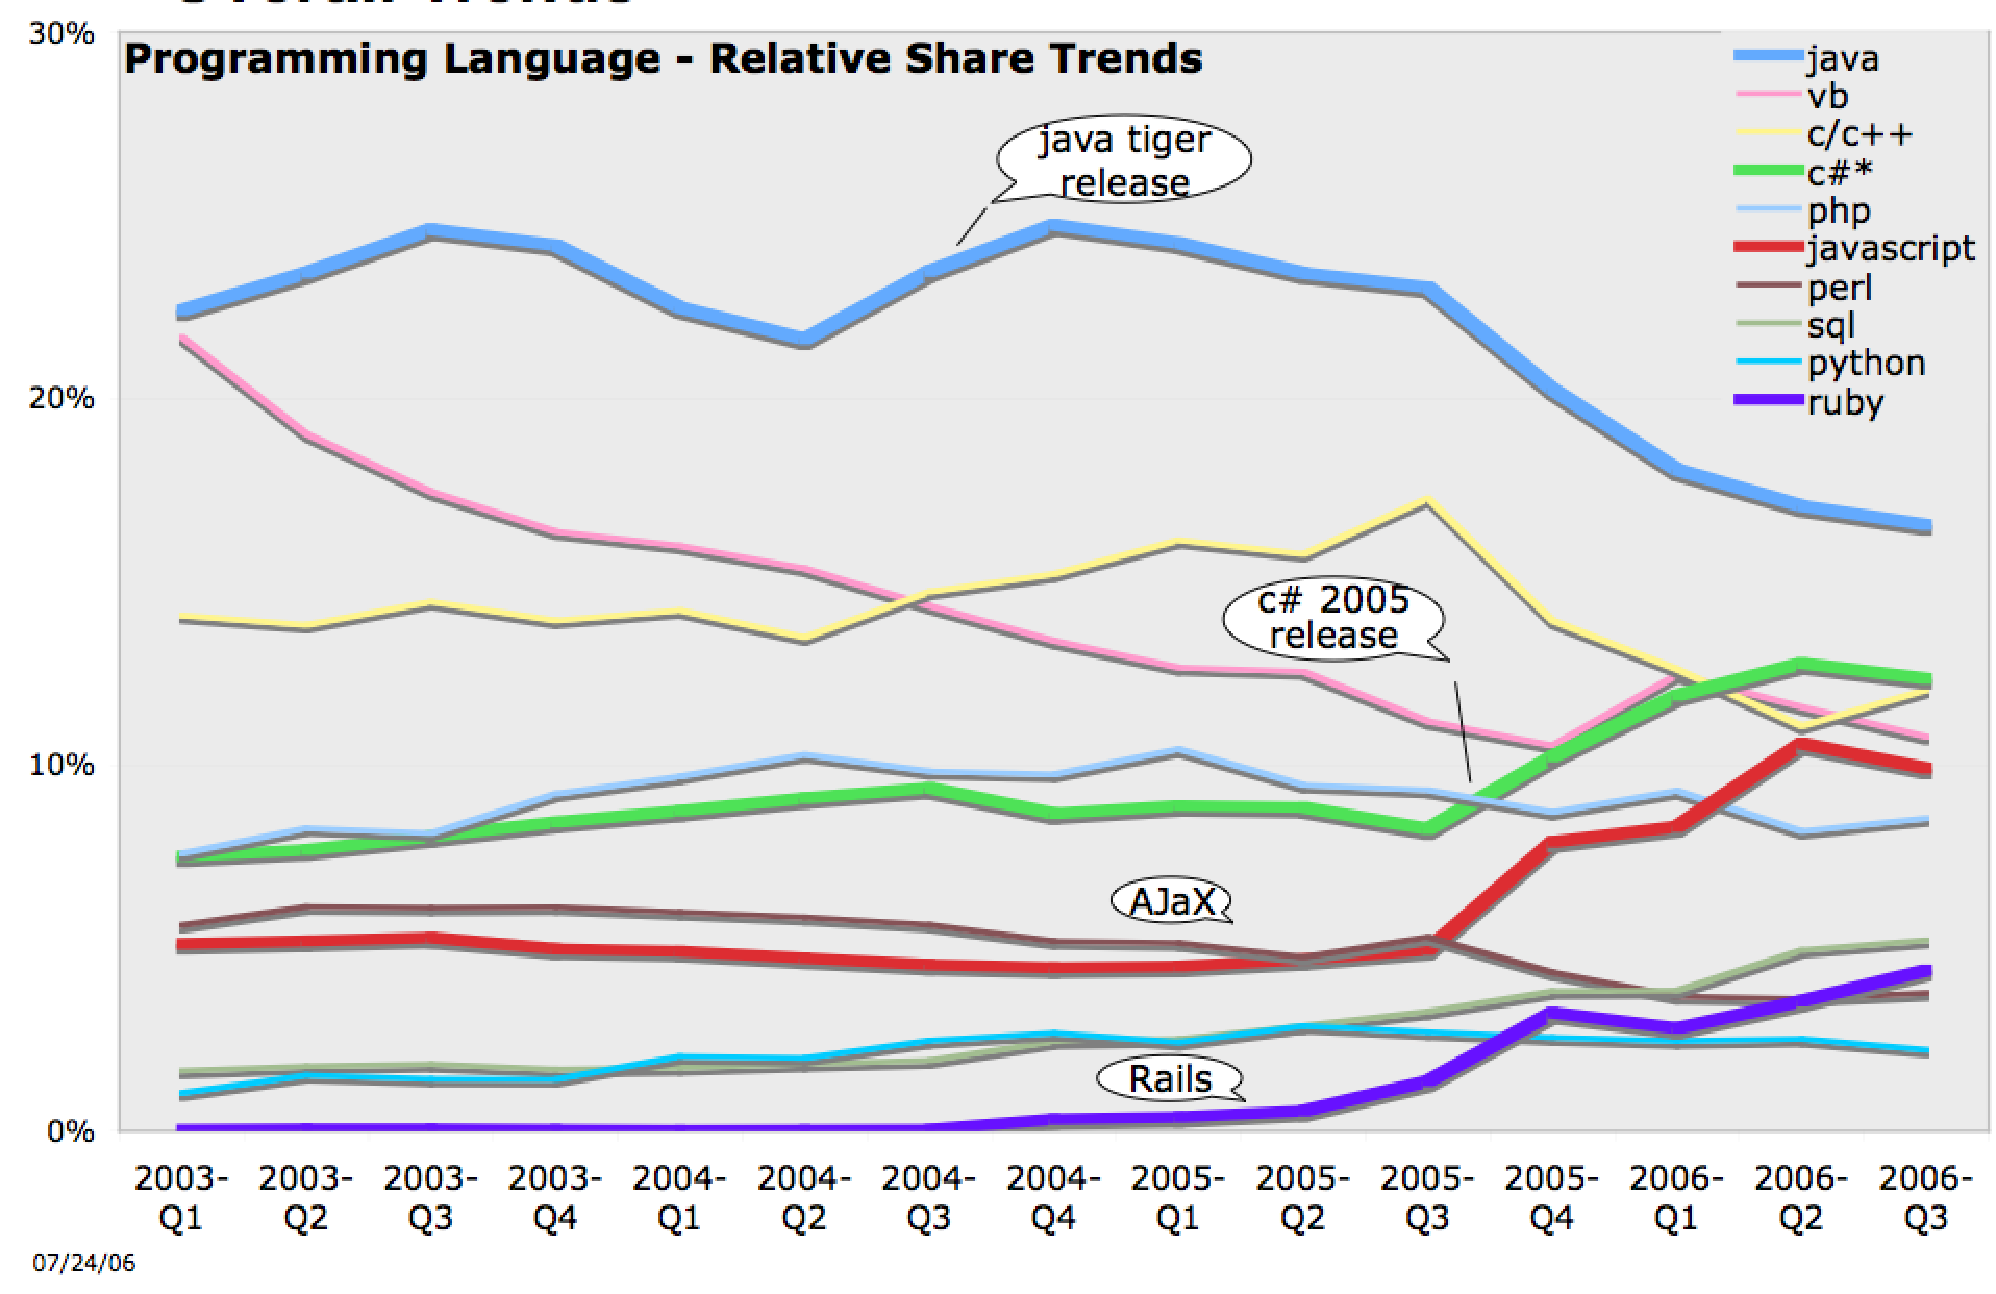
\includegraphics[width=0.85\linewidth]{figs/lang_distr.pdf}
	\end{figure}
\end{frame}


\begin{frame}
	\frametitle{Popularity of C in recent decade}
	\vspace{-0.1in}
	\begin{figure}
		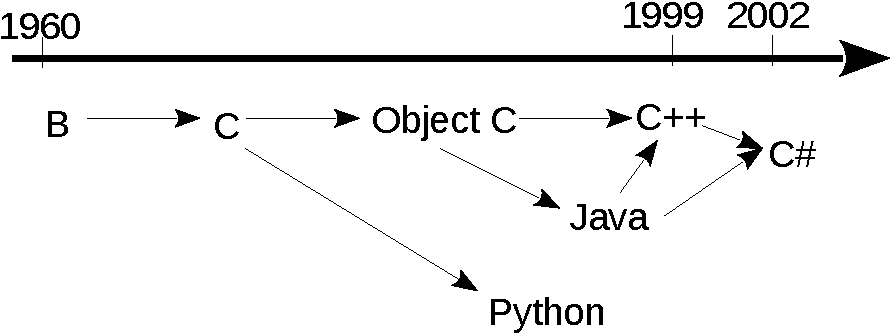
\includegraphics[width=0.85\linewidth]{figs/lag_evov.pdf}
	\end{figure}
\end{frame}



\section{}
\end{document}
